\section{Motivation and Problem Formulation}
\subsection{Why Local Substitution Fails}
A mesh snapshot feeds a mesh-specific publisher. If the snapshot tool fails,
an alternative producer may return a bridge payload for the same device.
Replacing only the producer breaks the consumer interface; replacing both can
preserve the output boundary and resume the unchanged continuation
(Fig.~\ref{fig:continuation-workflow}). The stopping point is therefore part of
the recovery decision. We write $f$ for the failed producer, $c$ for its
catalog-linked consumer, and $i,o$ for the immutable input and output ports.
For a fixed replacement assignment $\rho$, $R^*_{\rho}$ is its least
interface-closed repair region. A failure record $\xi$ contains the observed
failed input $a$, and $\mathcal{P}(\xi)$ denotes the compiled interface-closed
program set available at that failure.

The formal model covers an acyclic explicit dataflow. A port contract is a
predicate over explicit inputs, outputs, and failure outcomes. In the evaluated
read-only setting, an observable effect is the normalized value returned at an
immutable boundary; state-changing calls already committed to an external
system belong to $M$ and are never replaced. Online task completion is an
empirical endpoint rather than a consequence of the dataflow theorem.

ICR separates scope, compatibility, function, observed-value binding, and
input-conditional value preservation. Its packet carries the program, context,
and evidence; dispatch remains a separate authority decision.

\begin{figure*}[t]
\centering
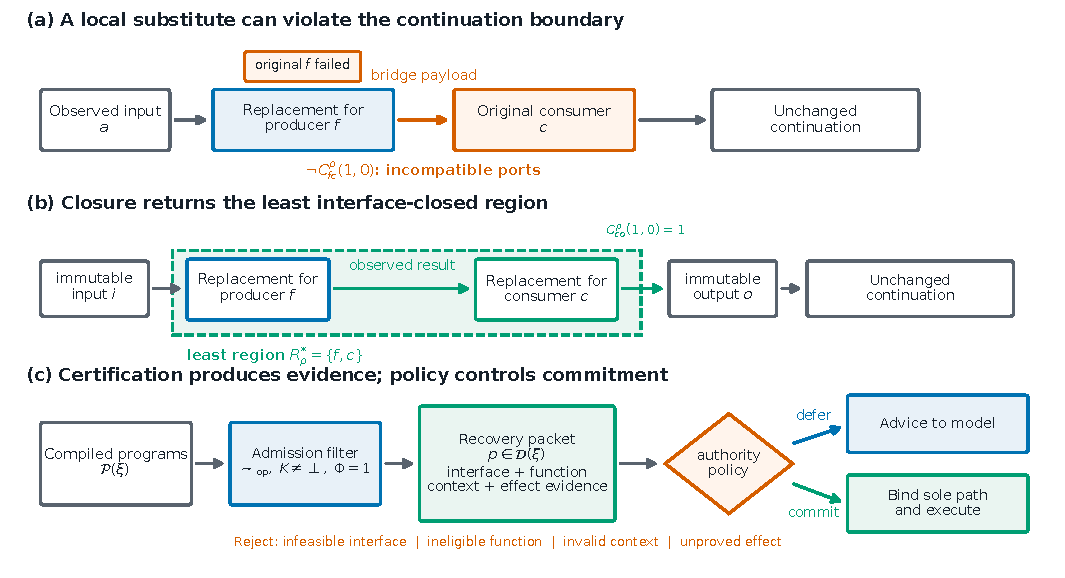
\includegraphics[width=.96\textwidth]{figures/continuation_workflow.pdf}
\caption{Interface-closed recovery from local substitution to a certified,
policy-gated continuation.}
\label{fig:continuation-workflow}
\end{figure*}

\subsection{Interface-Closed Region}
Let $G=(V,E)$ be an interface-valid workflow, $F\subseteq V$ the failed
required nodes, and $M\subseteq V$ the immutable nodes, including committed
effects and external ports. For a fixed candidate assignment $\rho$, each node
has its original or replacement implementation. For $(u,v)\in E$, let
$C^{\rho}_{uv}(b_u,b_v)$ indicate compatibility of the selected ports when
$b_u,b_v\in\{0,1\}$ choose the original implementation or the replacement
specified by $\rho$. The original graph satisfies $C^{\rho}_{uv}(0,0)$.

A repair region $R$ is feasible for $\rho$ if
\begin{equation}
 F\subseteq R\qquad R\cap M=\varnothing\qquad
 \bigwedge_{(u,v)\in E}C^{\rho}_{uv}(\mathbf{1}_{u\in R},\mathbf{1}_{v\in R})
 \label{eq:region-feasibility}
\end{equation}
The structural objective minimizes nonnegative node-change cost. Immutable
external ports preserve the unchanged interface. The least feasible region
under $\rho$ induces program $p_{\rho}$.
Let $\Phi(p_{\rho},a)$ denote boundary-value eligibility at the observed input and
$K(p_{\rho},\xi)$ the validated context, with $K(p_{\rho},\xi)=\bot$ on
validation failure. Structural closure enforces~\eqref{eq:region-feasibility};
admission also requires $\Phi(p_{\rho},a)=1$ and $K(p_{\rho},\xi)\ne\bot$.
